%FIX jan 9th, references in this chapter as well as comments
\chapter{Supersymmetry and the MSSM}
The standard model performs well in describing experimental observations at energies around
the electroweak scale of $O(246 \GeV)$.
The recent discovery of a standard model-like higgs boson ($m_{h}=$125 GeV) brings with it
more confidence in this theory. 
However, one must explain why the mass of the Higgs boson is as low as 125 GeV whereas
the planck scale is $O(1.22 \times10^{19} \GeV)$
\cite{Martin:1997ns}.
%However, questions arise when this model is seen as 
%a part of a grand unified theory, for example, what happens when we probe
%regions between the electroweak and planck scales $O(1.22 \times10^{19} \GeV)$? 
%The standard model encounters difficulties in renormalization, this is known
%as the Hierarchy Problem
%To illustrate these divergences we consider the radiative corrections to the higgs mass
%from a fermion loop.
%As seen in the previous chapter, 
%The potential of the standard model higgs field can be written as, 
%\begin{equation}
%V= \mu^{2}|\phi|^{2}+\lambda|\phi|^{4}
%\end{equation}
%where $\phi$ is a complex scalar field.
%A non-vanishing vacuum expectation value of $246 \GeV$ is required to derive the masses of the $W/Z$
%and the mass of the higgs which is defined as, $m_{h}=\sqrt{2\lambda v^{2}}$.

\begin{figure}[t]
  \centering
  \begin{subfigure}[trim = 0mm 0mm 0mm 0mm, clip, width=3cm]{.4\textwidth}
	\marginbox{0mm 0pt 0mm 0pt}{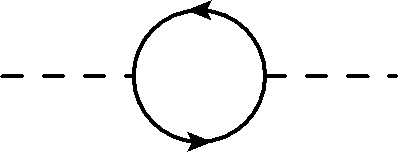
\includegraphics[width=\textwidth]{images/fermionLoop.png}}
                %\marginbox{-10mm 0pt 10mm 0pt}{}
                \caption{}
                \label{fig:fermionLoop}
\end{subfigure}
\begin{subfigure}[trim = 0mm 0mm 0mm 0mm, clip, width=3cm]{.4\textwidth}
	\marginbox{0mm 0pt 0mm 0pt}{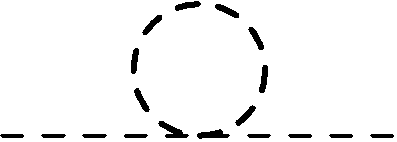
\includegraphics[width=\textwidth]{images/SLoop.png}}
	\caption{}
                %\marginbox{10mm 0pt -10mm 0pt}{}
                \label{fig:scalarLoop}
                	
  \end{subfigure}
   \caption[]{One loop quantum corrections for a fermion (\ref{fig:scalarLoop}) and a scalar (\ref{fig:scalarLoop}). }
\end{figure}

\section{Motivations for SUSY}
%When considering, for example, higher order radiative corrections to the mass of the higgs. For example, 
A fermion loop correction to $m_{h}$, seen in figure \ref{fig:fermionLoop}, 
%adds the term $-\lambda_{f}\phi \bar{f}f$ to the Lagrangian.
%This 
manifests as a negative-sign correction to the higgs mass, namely,
\begin{equation}
\Delta m_{H}^{2}=-\frac{|\lambda_{f}|^{2}}{8\pi^{2}}\Lambda_{UV}^{2}
\label{eq:SUS1}
\end{equation}
%The loops represent terms which are proportional to $m_{f}^{2}$.
where $\Lambda_{UV}$ is the ultraviolet high-mass cutoff, %%define UV cutoff
therefore, the correction to the higgs mass is large. 
%Then what happens when higher energy scales are considered and $\Lambda_{UV}\rightarrow \infty$?
%Since the standard model is a renormalizable theory one could simply
%pick $\Lambda_{UV}$ so that it regulates the loop. However, this would imply
%that $\Lambda_{UV}$ is the energy scale at which new physics should enter.
%To make matters worse, there are quantum corrections from the radiative
%effects of every particle that couples to the higgs. If each of these 
%particles gain their mass through the higgs mechanism then the entire standard model 
%mass spectrum is sensitive to $\Lambda_{UV}$!
It turns out that the correction due to a scalar loop,
as seen in figure \ref{fig:scalarLoop}, has an opposite sign to that of the fermion loop.
It is quite unnatural that the difference of two large numbers has to be tuned
carefully to obtain the 125 GeV observed Higgs boson mass. 
Supersymmetry supposes that there exists a scalar particle
for every fermion and vice versa. 
Therefore, this theory of symmetry between bosons
and fermions can naturally lead to a low mass higgs. 

%To solve the Hierarchy Problem suppose there exists a massive scalar particle S, 
%of mass $m_{S}$, that couples
%to the higgs with a term $-\lambda_{S}\phi^{2} S^{2}$ as seen is 
%figure \ref{fig:scalarLoop}. This massive scalar would give a correction of,
%\begin{equation}
%\Delta m_{H}^{2}=+\frac{\lambda_{s}}{16\pi^{2}}\left[\Lambda_{UV}^{2} \right].
%\label{eq:SUS2}
%\end{equation}
%By examining (\ref{eq:SUS1}) and (\ref{eq:SUS2}) it is apparent that if each of the quarks
%and leptons is accompanied by a complex scalar with $\lambda_{S}=|\lambda_{f}|^{2}$  %OR TWO??
%then the $\Lambda_{UV}^{2}$ terms will cancel. This model of symmetry between bosons
%and fermions is known as supersymmetry (SUSY).


To define SUSY a set of generators which 
transforms a fermionic state into a bosonic state and vice versa is needed. The simplest 
operator which can perform these operations is a 2 component Weyl spinor $Q$
such that,
\begin{equation}
Q|\mathrm{Boson}\rangle=|\mathrm{Fermion}\rangle \qquad Q|\mathrm{Fermion}\rangle=|\mathrm{Boson}\rangle.
\end{equation}
The generators $Q$ and $Q^{\dagger}$ must obey the anticommutation
and commutation algebra,
\begin{equation}
\{Q,Q^{\dagger}\}=P^{\mu}
\end{equation}
\begin{equation}
\{Q,Q\}=\{Q^{\dagger},Q^{\dagger}\}=0
\end{equation}
\begin{equation}
[P^{\mu},Q ]=[P^{\mu},Q^{\dagger}]=0
\end{equation}
where $P^{\mu}$ is the generator of space-time translations.

In the supersymmetric model the SM and SUSY particles are arranged
into supermultiplets. These supermultiplets must contain both the SM fermion
and the boson superpartner. In the simplest approach, a  spin $\frac{1}{2}$
weyl fermion (for example, $e$) must have %%%check this
a spin-0 superpartner ($\tilde{e}$), likewise, a supermultiplet 
with a spin-1 gauge boson ($W$) would have
 a spin $\frac{1}{2}$ weyl fermion superpartner ($\tilde{W}$).
The naming convention for super particles calls for the names of
the fermionic standard model particles to be prepended by an 's', for example, 
'selectron' is short of 'scalar electron'; the gauge bosons are appended
with an '-ino', for example $\tilde{W}$ is known as a 'wino'. If SUSY remained unbroken
then $m_{e}$ must be equal to $m_{\tilde{e}}$. Since sparticles like $\tilde{e}$ have not 
yet been discovered this implies that SUSY must be a broken
symmetry.

\section{Higgs Sector of the SM}
%%add in an introduction sentence

Electroweak
interactions happen on a very short range ($10^{-14}$ m).
To confine weak interactions to this
short range %fix?
the $W^{\pm}$ and Z bosons must be massive. %%need a transition sentence
However, the lagrangians governing fundamental interactions
of particles are written in terms of gauge symmetries and %fix
 in an unbroken gauge theory the gauge bosons must 
be massless. If one were to simply break the symmetry by adding 
in a mass term then the theory %%fix
would no longer be renormalizeable. Spontaneous Symmetry Breaking (SSB)
breaks the symmetry but still requires that the Lagrangian
is invariant under gauge transformations.  
This can done by introducing a complex $SU(2)_{L}$ doublet scalar
higgs field,
\begin{equation}
\Phi=\left(
    \begin{array}{c}
      \phi^{+} \\
      \phi^{0}
    \end{array}
  \right)
\end{equation}
This two component complex scalar field has four degrees
of freedom, three of them give mass to the $W^{\pm}$ and Z, the fourth
appears as a massive physical particle, the Standard Model Higgs boson. 
The Lagrangian describing interactions with this field is 
\begin{equation}
\La=(D_{\mu}\Phi^{\dagger})(D^{\mu}\Phi) +V(\Phi)
\end{equation}
where $D_{\mu}$ is a covariant derivative
and the scalar potential has the form,
\begin{equation}
V(\Phi)=\mu^{2}\Phi^{\dagger}\Phi+\frac{\lambda}{4}(\Phi^{\dagger}\Phi)^{2}.
\end{equation}
If $\lambda>0$ and $\mu^{2}>0$ then the shape of the potential is symmetric, however,
for  $\mu^{2}<0$ the minimum is a circle of radius $v$ where $v^{2}=-\mu^{2}/\lambda$.
Figure \ref{fig:mexicanHat} illustrates the shape of this potential. This is interpreted as
 a non-vanishing expectation value of the higgs field in the vacuum state.
The mass of the higgs boson is $m_{h}=\sqrt{2\lambda v^{2}}$. 
SSB generates mass for the both the gauge bosons and the fermions. Neglecting radiative corrections these are,
\begin{equation}
M_{W}=\frac{1}{2}gv, M_{Z}=\frac{\sqrt{g^{2}+g'^{2}}}{2} , m_{f}=\frac{G_{f}v}{\sqrt{2}}.
\end{equation}
The coupling between the higgs field and the 
massive gauge bosons is proportional to their mass squared while the coupling to the 
massive fermions is proportional to $m_{f}/v$. 

%To illustrate the Higgs mechanism 
%Conventional perturbation theory expands about a local minimum, therefore, 
%results in a massless Goldstone boson which has been converted to an
%additional longitudinal polarization degree of freedom. This results
%in a Lagrangian with a massive scalar particle, a massive field and interaction terms.
%This procedure is known as the Higgs mechanism. 

%Through couplings to the higgs field the gauge bosons a
%Finally and perturbations are considered around the new minimum. 

\begin{figure}[hb]
  \centering
	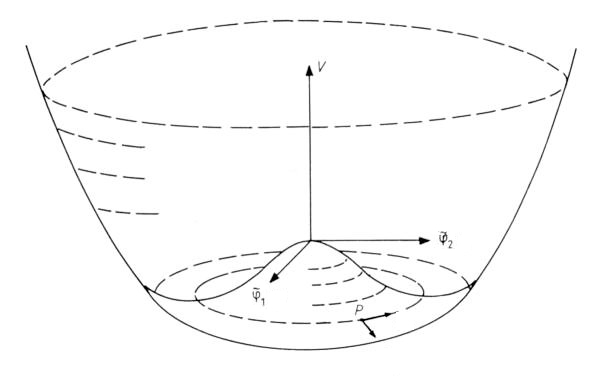
\includegraphics[width=0.5\textwidth]{images/mexicanHat.jpg}
  	\caption[Potential]
   	{$V(\phi)$ potential with $\lambda>0$ and $\mu^{2}<0$}
	\label{fig:mexicanHat}
\end{figure}

%In this section we illustrate the Higgs Mechanism and partially derive the
%Standard Model Lagrangian \cite{Halzen:1984mc}. 
%First we consider the Higgs Mechanism of a global gauge symmetry, 
%which is the mechanism that generates mass for the gauge bosons. 
%We start by writing the Lagrangian, 
%\begin{equation}
%\La=(\partial_{\mu}\phi)*(\partial^{\mu}\phi) - \mu^{2}\phi*\phi - \lambda (\phi*\phi)^{2}
%\label{eq:LU1}
%\end{equation}
%which describes the complex scalar field, $\phi=(\phi_{1}+i\phi_{2})/\sqrt{2}$.
%This Lagrangian is invariant under the phase transformation $\phi\rightarrow e^{i\alpha}\phi$
%(which is equivalent to stating that (\ref{eq:LU1}) possesses a $U(1)$ global gauge symmetry).
%Here, we consider the case where $\lambda>0$ and $\mu^{2}<0$. To illustrate the importance of (\ref{eq:LU1})
%this Lagrangian is rewritten in the form
%\begin{equation}
%\La \equiv T-V = \frac{1}{2}(\partial_{\mu}\phi_{1})^{2}+\frac{1}{2}(\partial_{\mu}\phi_{2})^{2}-\frac{1}{2}\mu^{2}(\phi_{1}^{2}+\phi_{2}^{2})-\frac{1}{4}\lambda(\phi_{1}^{2}+\phi_{2}^{2})^{2}.
%\label{eq:LU2}
%\end{equation}
%In (\ref{eq:LU2}) the potential term is
%\begin{equation}
%V=\frac{1}{2}\mu^{2}(\phi_{1}^{2}+\phi_{2}^{2})+\frac{1}{4}\lambda(\phi_{1}^{2}+\phi_{2}^{2})^{2}.
%\end{equation}
%Evaluating $\partial V/ \partial \phi = 0$ it is seen that the local minima
%of the potential $V(\phi)$ is a circle in the $\phi_{1},\phi_{2}$ plane of radius $v$ where,
%$\phi_{1}^{2}+\phi_{2}^{2}=v^{2}$ with $v^{2}= - \mu^{2}/\lambda$. This 
%is of great importance as $(\phi_{1},\phi_{2})=(0,0)$ is not the ground state, as can be seen in figure \ref{fig:mexicanHat}.
%Particle physics uses perturbation theory to calculate fluctuations 
%about the minimum energy so, without loss of generality, the field $\phi$ is translated to a minimum
%energy position $\phi_{1}=v$, $\phi_{2}=0$. The Lagrangian (\ref{eq:LU2}) is
%expanded about the vacuum in terms of the fields $\eta$, $\xi$ by substituting
%\begin{equation}
%\phi(x)=\sqrt{\frac{1}{2}}[v+\eta(x)+i\xi(x)]
%\label{eq:VTerms}
%\end{equation}
%into (\ref{eq:LU2}) and obtaining,
%\begin{equation}
%\La'=\frac{1}{2}(\partial_{\mu}\xi)^{2}+\frac{1}{2}(\partial_{\mu}\eta)^2+\mu^{2}+const.+\vartheta(\eta^{3},\xi^{3},\eta^{4},\xi^{4}).
%\label{eq:LU3}
%\end{equation}
%The third term of this new Lagrangian (\ref{eq:LU3}), is a mass term
%for the $\eta$-field, $m_{\eta}=\sqrt{-2\mu^{2}}$. The $\xi$-field has
%a kinetic term, the first term in (\ref{eq:LU3}), but no mass term
%for $\xi$. This is a consequence of the Goldstone theorem which states
%that whenever a symmetry is spontaneously broken, massless scalars occur.
%\begin{figure}[hb]
%  \centering
%	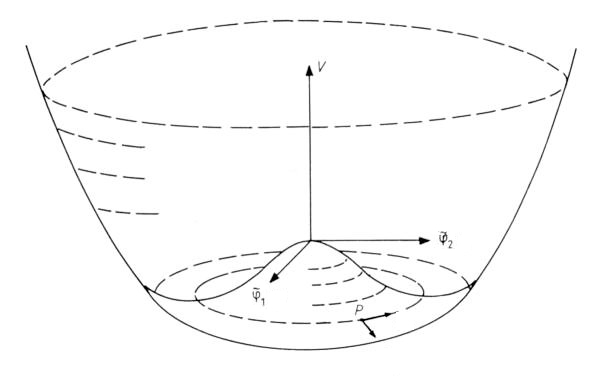
\includegraphics[width=0.5\textwidth]{images/mexicanHat.jpg}
%  	\caption[Potential]
%   	{$V(\phi)$ potential with $\lambda>0$ and $\mu^{2}<0$}
%	\label{fig:mexicanHat}
%\end{figure}
%
%Now that we have evaluated spontaneous breaking of 
%a global gauge symmetry we can extend the formalism to the local $U(1)$ gauge symmetry.
%First, we make the Lagrangian (\ref{eq:LU1}) invariant under a $U(1)$ 
%local gauge transformation: $\phi\rightarrow e^{i\alpha(x)}\phi$
%This is done by choosing a modified derivative, $D_{\mu}$, which will
%transform covariantly under phase transformations, namely, 
%$D_{\mu}\rightarrow e^{i\alpha(x)}D_{\mu}\psi$. Thus $\partial_{\mu}$
%is replaced by $D_{\mu} = \partial_{\mu}-ieA_{\mu}$.
%The gauge invariant Lagrangian in this instance is thus,
%\begin{equation}
%\La=(\partial^{\mu}+ieA^{\mu})\phi*(\partial_{\mu}-ieA_{\mu})\phi - \mu^{2} \phi*\phi - \lambda(\phi*\phi)^{2}-\frac{1}{4}F_{\mu\nu}F^{\mu\nu}.
%\end{equation}
%To avoid off diagonal terms, instead of making the transformation (\ref{eq:VTerms})
%we transform $\phi$ as,
%\begin{equation}
%\phi\rightarrow\sqrt{\frac{1}{2}}(\nu+h(x))e^{i\Theta(x)/\nu}
%\end{equation}
%and for the field $A_{\mu}$,
%\begin{equation}
%A_{\mu}\rightarrow A_{\mu}+\frac{1}{e\nu}\partial_{\mu}\Theta
%\end{equation}
%Then by translating this field to a true global minimum
%and, again, considering the solution where $\mu^{2}<0$ $\lambda>0$ this Lagrangian becomes 
%\begin{equation}
%\La'=\frac{1}{2}(\partial_{\mu}h)^{2}-\lambda \nu^{2}h^{2}+\frac{1}{2}e^{2}\nu^{2}A_{\mu}^{2}-\lambda\nu h^{3}-
%\frac{1}{4}\lambda h^{4} + \frac{1}{2}e^{2}A_{\mu}^{2}h^{2}+\nu e^{2}A_{\mu}^{2}h-\frac{1}{4}F_{\mu\nu}F^{\mu\nu}
%\end{equation}
%This equation describes the interaction between a vector gauge boson,
%$A_{\mu}$, and a massive scalar, h. 
%It is of importance to note that when examining this equation 
%we see that the second term relates the mass 
%of the higgs as $m_{h}=\sqrt{2\lambda v^{2}}$. 
%To summarize, this example of spontaneous breaking of a $U(1)$ gauge symmetry
%results in a massless Goldstone boson which has been converted to an
%additional longitudinal polarization degree of freedom. This results
%in a Lagrangian with a massive scalar particle, a massive field and interaction terms.
%This procedure is known as the Higgs mechanism. 
%
%Next we consider spontaneous breaking of a $SU(2)$ gauge symmetry.
%We begin with (\ref{eq:LU1}) and define $\phi$ as an $SU(2)$ doublet 
%of a complex scalar field, 
%\begin{equation}
%\phi=\left(
%    \begin{array}{c}
%      \phi_{\alpha} \\
%      \phi_{\beta}
%    \end{array}
%  \right) =
%  \sqrt{\frac{1}{2}} 
%  \left(
%    \begin{array}{c}
%      \phi_{1}+i\phi_{2} \\
%      \phi_{3}+i\phi_{4}
%    \end{array}
%  \right) .
%  \label{eq:phidoublet}
%\end{equation}
%We must replace $\partial_{\mu}$ by the covariant derivative,
%\begin{equation}
%D_{\mu}=\partial_{\mu}+ig\frac{\tau_{a}}{2}W_{\mu}^{a}.
%\end{equation}
%The gauge invariant Lagrangian finally becomes,
%\begin{equation}
%\La=
%\left(\partial_{\mu}\phi + ig \frac{1}{2} \tau \cdot W_{\mu}\phi  \right)^{\dagger}
%\left(\partial^{\mu}\phi + ig \frac{1}{2} \tau \cdot W^{\mu}\phi  \right)
%-\mu^{2}\phi^{\dagger}\phi
%-\lambda (\phi^{\dagger}\phi)^{2}
%-\frac{1}{4}W_{\mu\nu}W^{\mu\nu}.
%\label{eq:SU2L}
%\end{equation}
%Here, three gauge fields $W_{\mu}^{a}$ with a = 1,2,3 are included.
%The potential in this Lagrangian is $V(\phi)=\mu^{2}\phi^{\dagger}\phi+\lambda (\phi^{\dagger}\phi)^{2}$.
%As before, we are interested in the global minimum of this potential
%in the case where $\mu^{2}<0$ and $\lambda>0$, which is
%$\phi^{\dagger}\phi=-\mu^{2}/2\lambda$, and then we expand about a point in $\phi(x)$ that is a global minimum,
%\begin{equation}
%\phi_{0}=\sqrt{\frac{1}{2}}
%\left(
%\begin{array}{c}
%      0 \\
%      \nu
%    \end{array}
%\right)
%\label{eq:min}
%\end{equation}
%Due to gauge invariance, one can simply substitute,
%\begin{equation}
%\phi(x)=\sqrt{\frac{1}{2}}
%\left(
%\begin{array}{c}
%      0 \\
%      \nu+h(x)
%    \end{array}
%\right)
%\label{eq:min}
%\end{equation}
%And in fact, if we substitute ($\ref{eq:min}$) into the Lagrangian (\ref{eq:SU2L}).
%we find that the three bosons acquire a mass of $M=\frac{1}{2}gv$.
%
%Finally, we need to formulate the Higgs mechanism in an $SU(2)\times U(1)$ 
%gauge invariant Lagrangian so that the $W^{\pm}$ and $Z$ become massive. 
%\begin{equation} %%link this to 14.65
%\left| \left( i\partial_{\mu}+gT_{a}W_{\mu}^{1}+g'B_{\mu}\frac{Y}{2}\right)\phi \right|^{2} - \mu^{2}\left| \phi \right| ^{2}
%-\lambda\left| \phi \right| ^{4}
%\label{eq:L2}
%\end{equation}
%%%%%delete
%We wish for (\ref{eq:L2}) to remain gauge invariant and 
%for this Lagrangian to break the symmetries of $SU(2)$ and $U(1)_{Y}$
%but leave $U(1)_{em}$, with generator $Q=T^{3}+\frac{Y}{2}$, unbroken. 
%We can then make the same choice of (\ref{eq:phidoublet}) and require a vacuum 
%expectation value of (\ref{eq:min}).
%
%Expanding the kinetic term of (\ref{eq:L2}) we have,
%\begin{equation}
%\left| \left(-g\frac{\tau}{2}\cdot W_{\mu}-i\frac{g'}{2}B_{\mu}\right)\phi\right|^{2}
%\end{equation}
%Then evaluating at (\ref{eq:min}),
%\begin{equation}
%=\frac{1}{8}\left|
%\begin{pmatrix}
%		gW_{\mu}^{3}+g'B_{\mu} & g(W_{\mu}^{1}-iW_{\mu}^{2})\\
%		g(W_{\mu}^{1}+iW_{\mu}^{2}) & -gW_{\mu}^{3}+g'B_{\mu}
%\end{pmatrix}
%\begin{pmatrix}
%0\\
%\nu
%\end{pmatrix}
%\right|^{2}
%\end{equation}
%\begin{equation}
%=
%\frac{1}{8}v^{2}g^{2}\left[\left(W_{\mu}^{1} \right)^{2} \left(W_{\mu}^{2} \right)^{2} \right]
%+\frac{1}{8}v^{2}(g'B_{\mu}-gW_{\mu}^{3})(g'B^{\mu}-gW^{3\mu}) 
%\end{equation}
%\begin{equation}
%=(\frac{1}{2}v g)W_{\mu}^{+}W^{-\mu}+\frac{1}{8}(W_{\mu}^{3},B_{\mu})
%\begin{pmatrix}
%g^{2} & -gg'\\
%-gg'  & g'^{2}
%\end{pmatrix}
%\begin{pmatrix}
%W^{3\mu}\\
%B^{\mu}
%\end{pmatrix}
%\label{eq:finalH}
%\end{equation}
%We then can obtain the masses of the vector bosons.
%From the first term in (\ref{eq:finalH}) we can then determine the 
%mass of the $W$ boson, 
%\begin{equation}
%M_{W}=\frac{1}{2}v g.
%\end{equation}
%By diagonalizing the matrix on the last term of (\ref{eq:finalH}), we find that
%the field associated to $Z_{\mu}$ is,
%\begin{equation}
%Z_{\mu}= \frac{gW_{\mu}^{3}-g'B_{\mu}}{\sqrt{g^{2}+g'^{2}}}
%\end{equation}
%and therefore we have,
%\begin{equation}
%M_{Z}=\frac{1}{2}v\sqrt{g^{2}g'^{2}}.
%\end{equation}
%While it is not required in the standard model that the higgs boson 
%also gives mass to the fermions, it is possible and would be a nice
%feature. If this were true then the coupling strength to each of the fermions
%to the higgs boson would be proportional to their mass.
%
%To generate (for example) the $\tau$ mass we construct a 
%Lagrangian that is $SU(2)\times U(1)$ gauge invariant,
%
%\begin{equation}
%\La = -G_{\tau}\left[
%      (\bar{\nu_{\tau}},\bar{\tau})_{L}
%	\left( \begin{array}{c}
%      \phi^{+} \\
%      \phi^{-}
%      \end{array}\right)\tau_{R} 
%    +
%      \bar{\tau}_{R}(\phi^{-},\bar{\phi^{0}})
%	\left( \begin{array}{c}
%      \nu_{e} \\
%      e
%      \end{array}\right)_{L}
%    \right]
%\end{equation}
%Substituting in
%\begin{equation}
%\phi=\sqrt{\frac{1}{2}}
%\left( \begin{array}{c}
%      0 \\
%      \nu + h(x)
%      \end{array}\right)
%\end{equation}
%This leads to,
%\begin{equation}
%\La = -\frac{G_{\tau}}{\sqrt{2}}\nu(\bar{\tau}_{L}\tau_{R}+\bar{\tau}_{R}\tau_{L})
%-\frac{G_{\tau}}{\sqrt{2}}(\bar{\tau}_{L}\tau_{R}+\bar{\tau}_{R}\tau_{L})h.
%\end{equation}
%Then the masses of the fermions can be obtained by choosing $G_{e}$ such that,
%\begin{equation}
%m_{e}=\frac{G_{e}\nu}{\sqrt{2}}
%\end{equation}
%The recent evidence of $h$ coupling to $\tau\tau$ (REFERENCE PAPER) suggests
%that the higgs mechanism could be used to give mass to the fermions, however,
%it is not required and more measurements will need to be performed.

\section{Higgs Sector of the MSSM}
\label{sec:HiggsMSSM}
The most simple supersymmetric extension of the standard model is the MSSM.
In the MSSM there are two higgs doublets with an $SU(2)_{L}$ symmetry,
\begin{equation}
\Phi_{1}=
\left(
    \begin{array}{c}
      \phi_{1}^{0*} \\
      -\phi_{1}^{-}
    \end{array}
  \right) 
 \qquad
\Phi_{2}=
\left(
    \begin{array}{c}
      \phi_{2}^{+} \\
      -\phi_{2}^{0}
    \end{array}
  \right), 
  \label{eq:SUSYhiggs}
\end{equation}
The $\Phi_{1}$ has a hypercharge of -1 and gives mass to each of the
down-type quarks and charged leptons whereas $\Phi_{2}$ gives masses
to the up-type quarks. The extra doublet
is needed to cancel out the corresponding supersymmetric higgs fermion
contributions.
$H_{1}^{0}$ and $H_{2}^{0}$ acquire vacuum expectation values $v_{1}$ and $v_{2}$ where
\begin{equation}
v = \sqrt{2}(v_{1}^{2}+v_{2}^{2})^{\frac{1}{2}}.
\end{equation}
The ratios of $v_{1}$ and $v_{2}$ is written as,
\begin{equation}
\tan(\beta)=\frac{v_{2}}{v_{1}}
\end{equation}
%%% something about shifting the neutral scalar fields by their vevs and diagonalization 
%The following higgs boson states are attained
Consequently the MSSM model has a total of five higgs bosons: two neutral higgs, h and H,
a pseudoscalar, A, and two charged higgs, $H^{\pm}$.
By translating the fields in (\ref{eq:SUSYhiggs}) to their minima and diagonalizing the matrix
the following higgs boson states are obtained,
\begin{equation}
\left(
    \begin{array}{c}
      H^{0}_{1} \\
     H^{0}_{2}
    \end{array}
  \right) 
  =
  \sqrt{2}
  \begin{pmatrix}
  \cos{\alpha} & \sin{\alpha}\\
  -\sin{\alpha}& \cos{\alpha}\\
  \end{pmatrix}
\left(
      \begin{array}{c}
      Re{\phi}_{1}^{0*}-v_{1} \\
     Re{\phi}_{2}^{0}-v_{2}
    \end{array}
  \right) 
\end{equation}
\begin{equation}
H_{3}^{0}=\sqrt{2}(\sin{\beta}Im\phi_{1}^{0*}+\cos{\beta}Im\phi^{0}_{2})
\end{equation}
\begin{equation}
H^{-}=(H^{+})^{*}=-\phi_{1}^{-}\sin{\beta}+\phi_{2}^{-}\cos{\beta}
\end{equation}

In the MSSM at tree level the number of independent parameters can be reduced to 3: $m_{W}$,
$\tan{\beta}$ and the mass of the pseudoscalar, $m_{A}$. The neutral boson masses are,
\begin{equation}
m_{h}^{2}=\frac{1}{2}\left(m_{A}^{2}+M_{Z}^{2}-\left[(m_{A}^{2}+
M_{Z}^{2})^{2}-4M_{Z}^{2}m_{A}^{2}\cos^{2}{(2\beta)}\right]^{\frac{1}{2}}\right)
\end{equation}
\nobreak
\begin{equation}
m_{H}^{2}=\frac{1}{2}\left(m_{A}^{2}+M_{Z}^{2}+\left[(m_{A}^{2}+
M_{Z}^{2})^{2}-4M_{Z}^{2}m_{A}^{2}\cos^{2}{(2\beta)}\right]^{\frac{1}{2}}\right).
\end{equation}
While the masses of the two charged bosons are,
\begin{equation}
m_{H^{\pm}}^{2}=m_{A}^{2}+M_{W}^{2}.
\end{equation}
In order to make reliable phenomenological predictions, loop corrections must be included
which depend on the particle masses and free parameters of the SUSY model.
Due to the large number of free parameters,
searches for MSSM Higgs bosons are expressed in terms of benchmark scenarios where 
the lowest-order parameters tan$\beta$ and $M_A$ are varied, while fixing the other parameters that 
enter through radiative corrections to benchmark values. 
The $m_{h}^{\rm max}$ scenario~\cite{MHMAX-Carena,MHMAX-Carena-2002}
yields expected limits in the tan$\beta$ and $M_A$ plane. %%%FIX here JAN 9TH
The following parameters are fixed in the $m_{h}^{\rm max}$ scenario:
\begin{center}
$
M_{SUSY} = 1 \mathrm{TeV}, 
\mu=-200 \mathrm{GeV}, 
$
\linebreak[4]
$
m_{\tilde{g}}=0.8 M_{SUSY}, 
M_{A} \leq 1000 \mathrm{GeV}, 
$
\linebreak[4]
$
X_{t}=2M_{SUSY}, 
A_{b} = A_{t}
$
%\linebreak[4]
\end{center}
where 
$M_{SUSY}$ is the third generation squark mass parameter,
$\mu$ is the higgsino mass parameter,
$m_{\tilde{g}}$ is the gluino mass,
$X_{t}= A_{t}-\mu/\mathrm{tan}\beta$
$A_{b}$ denotes the higgs-sbottom coupling and
$A_{t}$ is the trilinear higgs-stop coupling.
The gaugino mass parameter, $M_{1}$, is fixed via the GUT relation,
\begin{equation} 
M_{1}=\frac{5\sin^{2}{\theta_{w}}}{3\cos^{2}{\theta_{w}}}M_{2}
\end{equation}
where $M_{2}$ is the SU(2)-gaugino mass parameter.
Results in this thesis are interpreted both in the context of the MSSM 
$m_{h}^{\rm max}$ scenario and also in a model independent way, 
in terms of upper limits on $\sigma\cdot$BR($A\slash H\slash h\rightarrow\Pgt\Pgt$) for 
gluon-fusion and b-associated neutral higgs boson production.

\section{MSSM Higgs Production}

\begin{figure}[t]
\centering
  \begin{subfigure}[b]{.4\textwidth}
	\marginbox{-5mm 10pt 5mm 0pt}{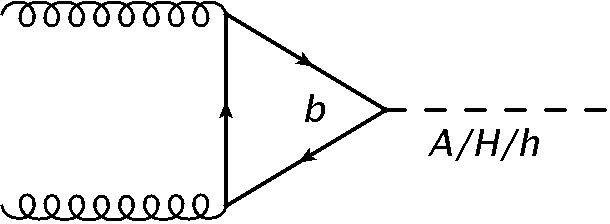
\includegraphics[width=\textwidth]{images/ggA.png} }
\caption[]{}
	\label{fig:ggA}
	\end{subfigure}	
   \begin{subfigure}[b]{.4\textwidth}
	\marginbox{5mm 0pt -5mm 0pt}{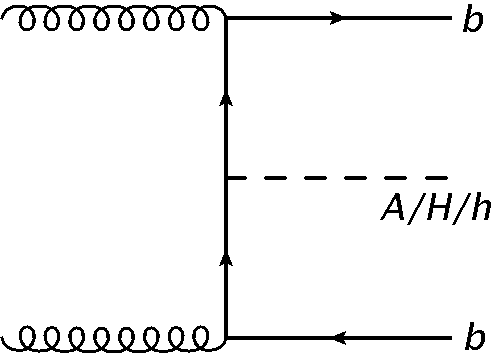
\includegraphics[width=\textwidth]{images/bbA.png}}
	\label{fig:bbA}
	\caption[]{}
    \end{subfigure}	
  	\caption[]
   	{MSSM Higgs Production diagrams}
	\label{fig:MSSMdiagrams}
\end{figure}
The two higgs doublet model of the MSSM is responsible for interesting
phenomenological effects which do not occur in the SM.
The dominant production mechanisms for the higgs particles are gluon
fusion and associated production of b quarks. 
The neutral MSSM Higgs boson production cross section
for small and moderate values of tan$\beta$ is high for 
gluon fusion ($gg\rightarrow A/H/h$) shown in figure (\ref{fig:MSSMdiagrams}a). 

At large values of tan$\beta$ 
the b-associated production is the dominant contribution due to the enhanced bottom Yukawa 
coupling; therefore, associated production of b quarks with $A/H/h$ becomes a dominant signature.
Production of $gg\rightarrow A/H/h+bb$ is shown in figure (\ref{fig:MSSMdiagrams}b). 
Identification of a b jet in the final state also serves to reduce further unwanted backgrounds
such as $Z\rightarrow \Pgt\Pgt$. 

Figure (\ref{fig:tanbeta}a) shows cross sections for various MSSM higgs boson 
production mechanisms at a value of $\tan\beta=5$ and figure (\ref{fig:tanbeta}b)
shows them at $\tan\beta=30$.
Performing an analysis with and without b jet associated
production is useful for probing a larger region of MSSM phase space. Futhermore, due to
recently improved 
$\tau$ identification techniques developed at CMS \cite{CMS-PAS-TAU-11-001} 
and enhanced couplings to $\tau$ and b-quarks 
the search for $A/H/h\rightarrow \Pgt\Pgt$ 
at the LHC is of particular interest and will continue to be an important
mode for MSSM discovery into the 2015 run.

\begin{figure}[hb]
\centering
  \begin{subfigure}[b]{.4\textwidth}
	\marginbox{-5mm 10pt 5mm 0pt}{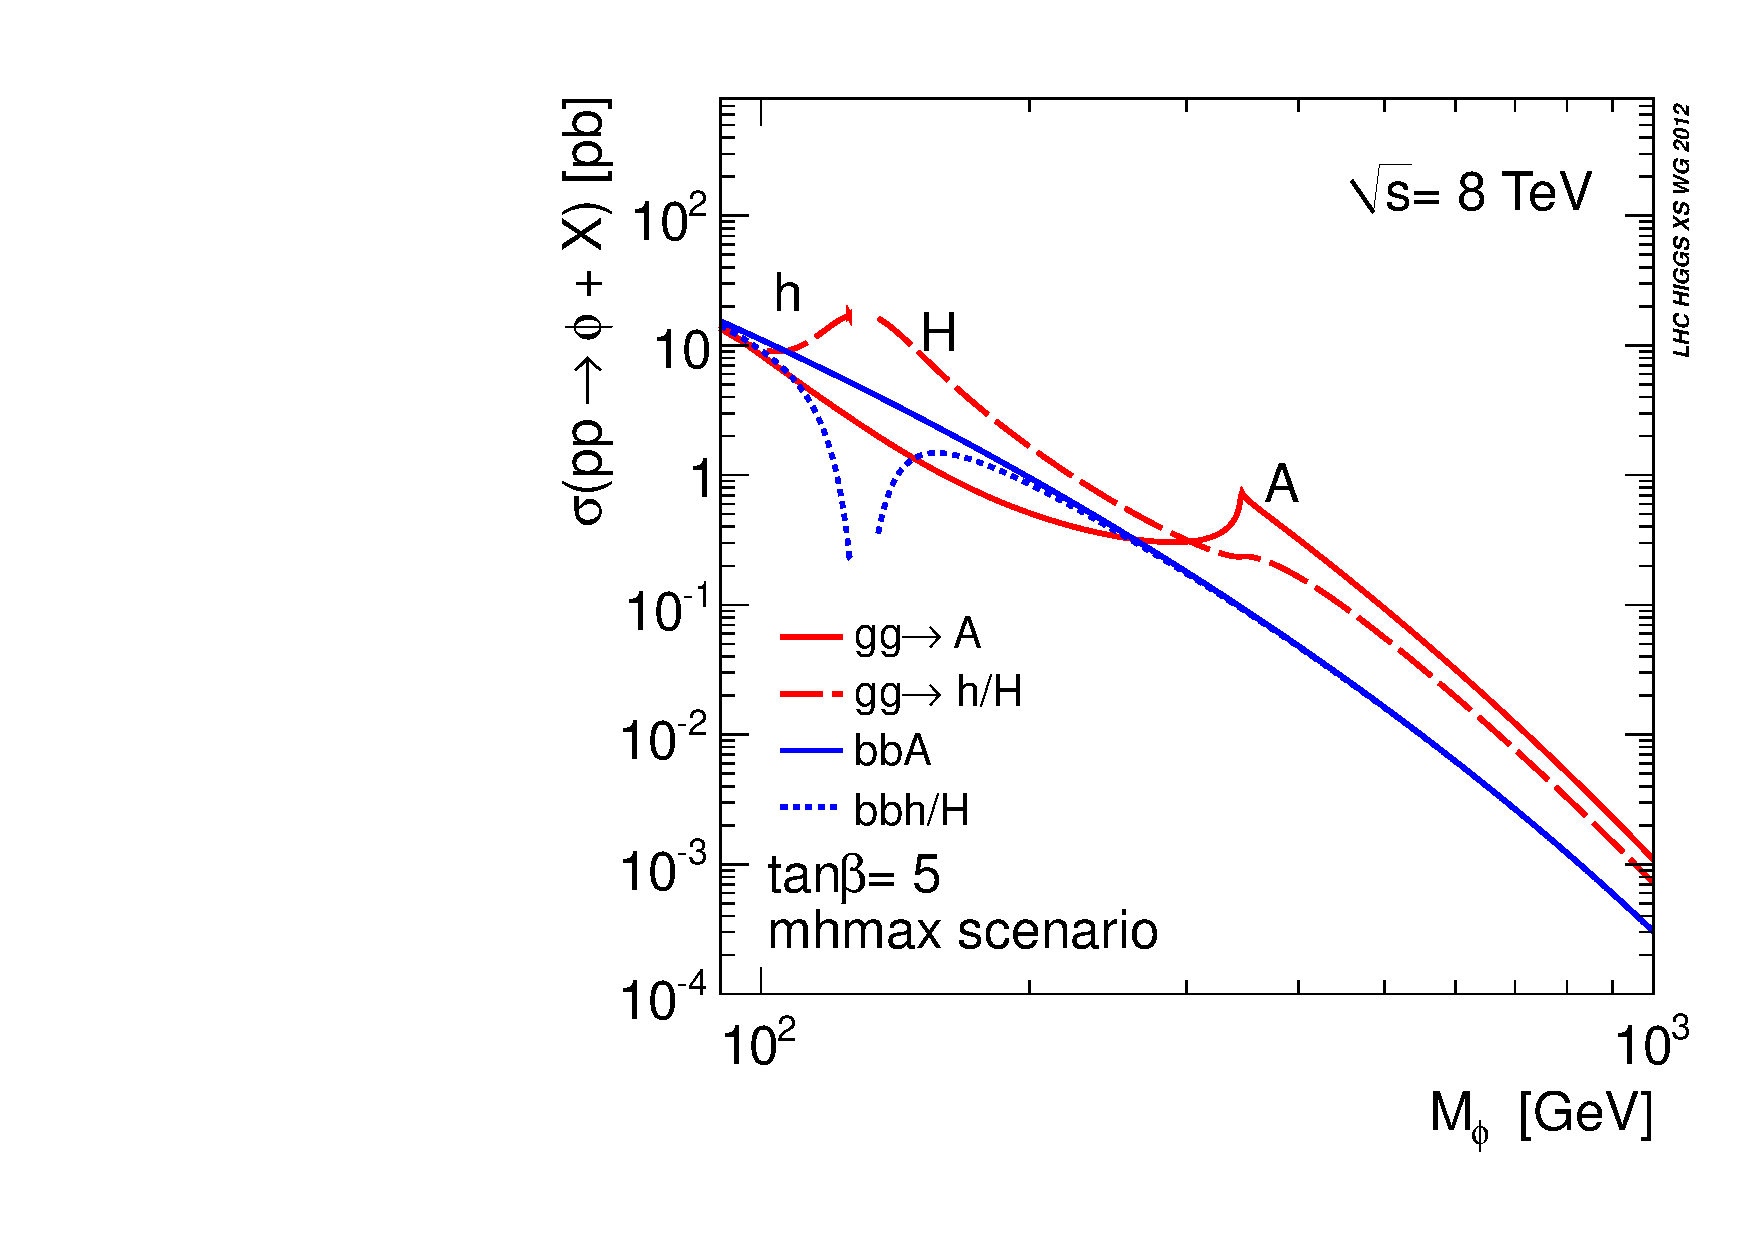
\includegraphics[width=\textwidth]{images/tanbeta5.pdf}}
	\label{fig:tanbeta5}
	\caption[]{$\tan\beta=5$}
	\end{subfigure}	
   \begin{subfigure}[b]{.4\textwidth}
	\marginbox{5mm 0pt -5mm 0pt}{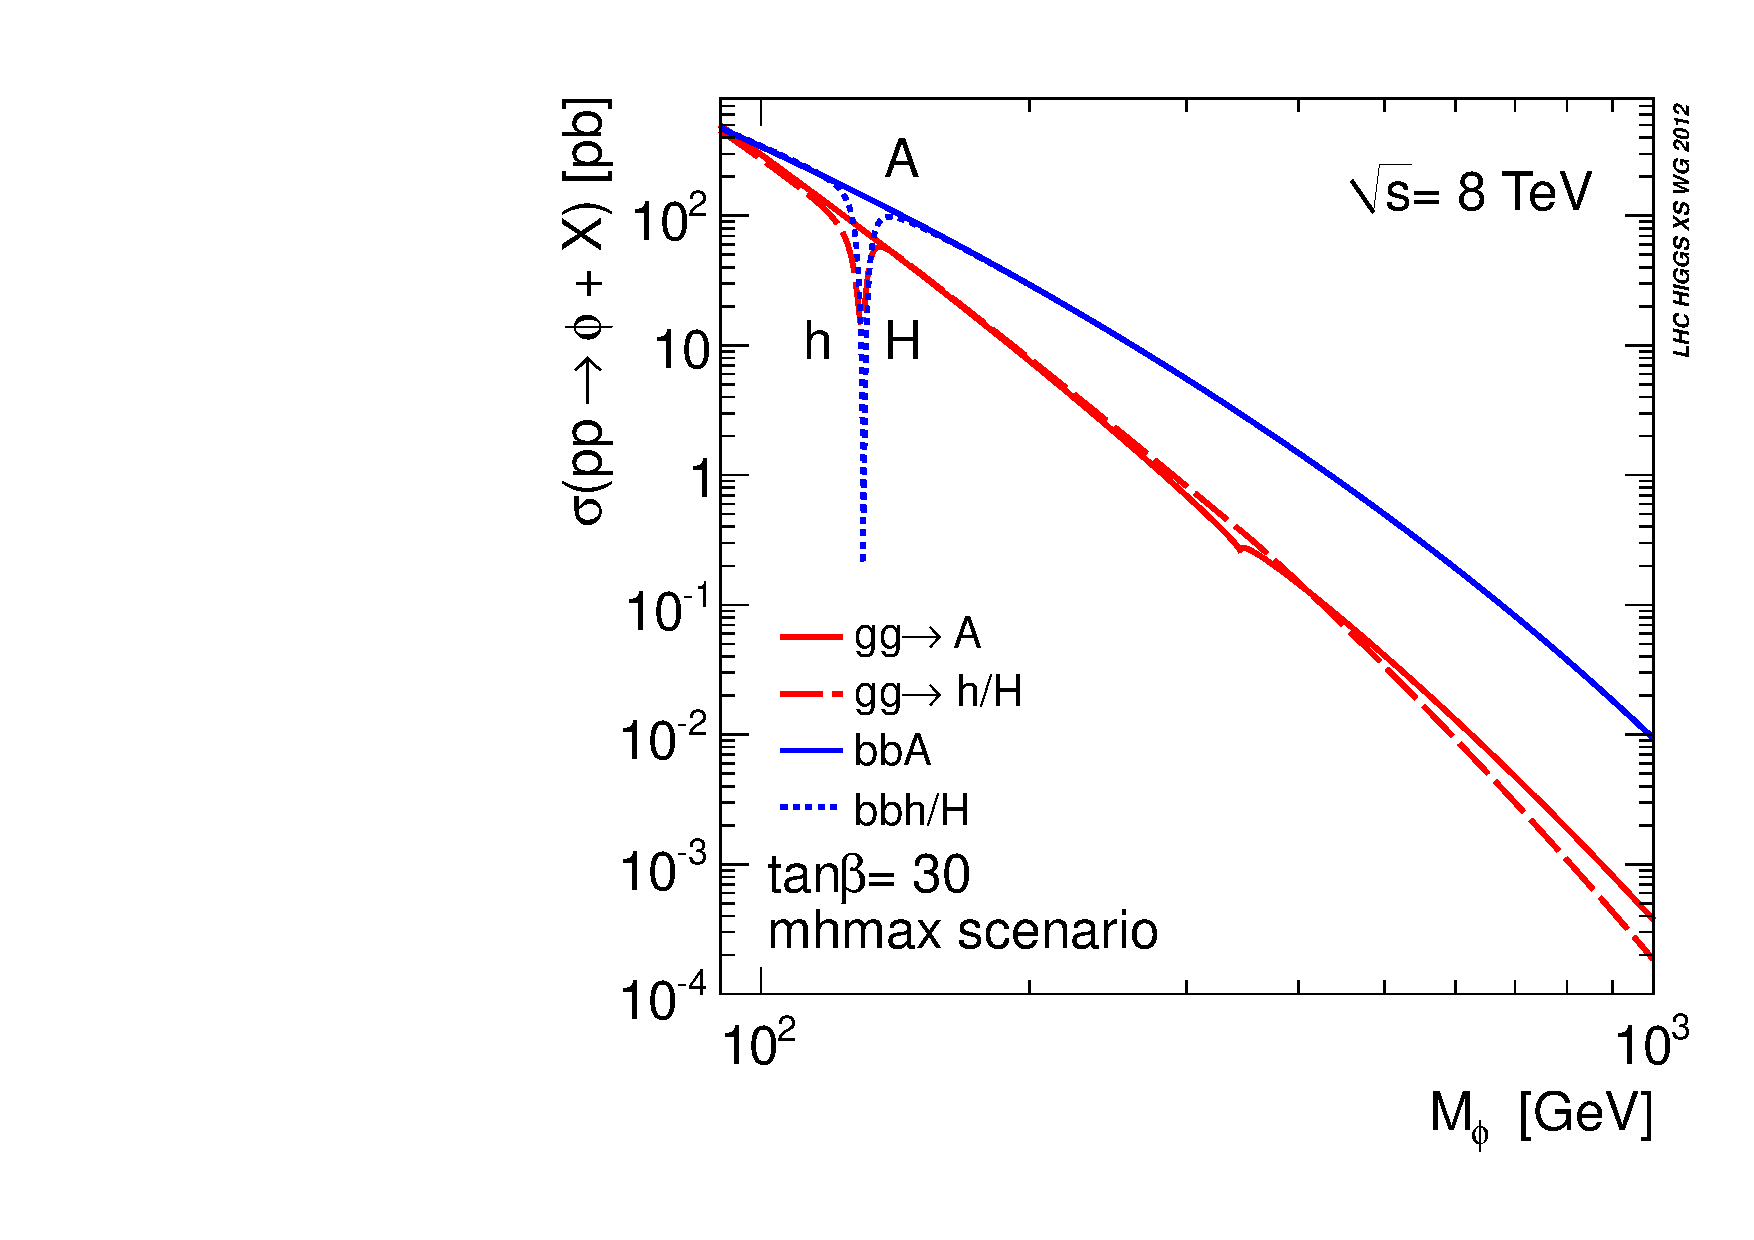
\includegraphics[width=\textwidth]{images/tanbeta30.pdf}}
	\caption[]{$\tan\beta$=30}
	\label{fig:tanbeta30}
    \end{subfigure}	

  \caption[]
   	{The cross sections for various MSSM higgs bosons and production 
	mechanisms at 8 TeV \cite{LHCHiggsCrossSectionWorkingGroup:2011ti}}
    \label{fig:tanbeta}
\end{figure}

%making the search for neutral MSSM Higgs bosons in the di-$\Pgt$ final state of particular interest. 
%In the region of large tan$\beta$, $O(10)$, the coupling to the heaviest down type fermions 
%$(b,\Pgt)$ is enhanced, 




